\chapter{Abstraktion und Struktur}
\label{chap:VI_abstraktion}



\subsection{Einleitung}

In den vorhergehenden Kapiteln wurde gezeigt, dass Naturgesetze\index{Naturgesetz} nicht durch anschauliche Bilder, sondern durch mathematische Beziehungen beschrieben werden. Bewegung\index{Bewegung}, Wachstum\index{Wachstum} und Dynamik\index{Dynamik} lassen sich nur verstehen, wenn Veränderung\index{Veränderung} formal gefasst wird. Damit stellt sich eine weiterführende Frage: Wie ist es möglich, dass abstrakte mathematische Begriffe reale Naturphänomene so präzise erfassen?

Die Antwort liegt im Prinzip der Abstraktion\index{Abstraktion}. Mathematik\index{Mathematik} verzichtet bewusst auf viele Eigenschaften der Wirklichkeit, um ihre strukturellen Eigenschaften freizulegen. Sie beschreibt nicht, \emph{was} ein Objekt ist, sondern \emph{wie} es sich verhält und in Beziehung zu anderen Objekten steht. Abstraktion ist dabei kein Verlust an Realität\index{Realität}, sondern eine gezielte Reduktion auf das Wesentliche.

Struktur\index{Struktur} bezeichnet genau das, was unter dieser Reduktion erhalten bleibt. Sie ist unabhängig vom konkreten Material, vom Maßstab oder vom Ort\index{Ort}. Ob ein System aus Punkten, Teilchen\index{Teilchen} oder Feldern\index{Feld} besteht, ist für die mathematische Struktur zunächst unerheblich. Entscheidend ist allein das Beziehungsgeflecht, das diese Elemente verbindet.

Dieses Kapitel untersucht, wie Abstraktion und Struktur zusammenwirken und warum sie der Schlüssel zum Verständnis moderner Mathematik und Physik\index{Physik} sind. Es zeigt, dass Mathematik nicht deshalb erfolgreich ist, weil sie die Wirklichkeit imitiert, sondern weil sie ihre Strukturen freilegt.

\subsection{Vektoren und Räume}

Der Begriff des Vektors\index{Vektor} gehört zu den bekanntesten Elementen der Mathematik\index{Mathematik} und Physik\index{Physik}. Im schulischen Kontext erscheint er meist als Pfeil: mit Richtung, Länge und Orientierung. Diese Vorstellung ist hilfreich, aber sie trifft nicht den Kern. Ein Vektor ist nicht in erster Linie ein geometrisches Objekt, sondern ein abstraktes Element eines Raumes\index{Raum}.

Diese Verschiebung der Perspektive ist entscheidend. Mathematik interessiert sich nicht dafür, wie ein Vektor aussieht, sondern dafür, wie er sich zu anderen Vektoren verhält. Addition\index{Addition}, Skalierung\index{Skalierung} und Vergleich sind keine Rechentricks, sondern grundlegende Strukturmerkmale. Erst durch diese Beziehungen wird ein Raum mathematisch definiert.

Ein Raum ist daher nicht einfach eine Menge von Punkten\index{Punkt}. Er ist ein System von Beziehungen\index{Relation}, in dem bestimmte Operationen sinnvoll definiert sind. Welche Objekte diesen Raum bilden, ist zunächst zweitrangig. Vektoren können Verschiebungen\index{Verschiebung} im Raum darstellen, Geschwindigkeiten\index{Geschwindigkeit}, Kräfte\index{Kraft}, Zustände\index{Zustand} oder abstrakte Informationsinhalte. Entscheidend ist nicht ihre Bedeutung, sondern die Struktur\index{Struktur}, die sie gemeinsam besitzen.

Gerade hier zeigt sich die Kraft der Abstraktion\index{Abstraktion}. Indem Mathematik von der konkreten Interpretation absieht, werden völlig unterschiedliche Phänomene vergleichbar. Der gleiche Vektorraum\index{Vektorraum} kann Bewegungen beschreiben, elektrische Felder\index{Feld} strukturieren oder Zustände in der Quantenmechanik\index{Quantenmechanik} repräsentieren. Was sich ändert, ist die physikalische Deutung – nicht die mathematische Form.

Diese Sichtweise kehrt die gewohnte Denkweise um. Nicht der Raum ist durch seine Elemente bestimmt, sondern die Elemente erhalten ihre Bedeutung durch den Raum, in dem sie liegen. Ein Vektor ist nicht „an sich“ ein Pfeil, sondern wird erst durch die Struktur des Raumes zu dem, was er ist. Abstraktion bedeutet hier nicht Verzicht, sondern Präzisierung.

Die Einführung von Vektorräumen markiert daher einen Wendepunkt. Mathematik löst sich von anschaulichen Bildern und formuliert Strukturen, die unabhängig von Dimension\index{Dimension}, Maßstab oder physikalischem Kontext gültig sind. Ein Raum kann endlich oder unendlich dimensional sein, kontinuierlich oder diskret. Die formalen Beziehungen bleiben dieselben.

Damit wird verständlich, warum moderne Physik\index{Moderne Physik} ohne diese abstrakten Räume nicht auskommt. Felder sind keine Sammlungen von Zahlen, sondern Elemente geeigneter Funktionsräume\index{Funktionsraum}. Quantenzustände sind keine Bahnen, sondern Vektoren in abstrakten Zustandsräumen\index{Zustandsraum}. Die Wirklichkeit\index{Wirklichkeit} wird nicht geometrischer, sondern relationaler beschrieben.

Vektoren und Räume sind somit kein technisches Hilfsmittel, sondern ein grundlegendes Denkwerkzeug. Sie zeigen exemplarisch, wie Mathematik Wirklichkeit nicht abbildet, sondern strukturiert. Abstraktion ist hier nicht das Entfernen von Realität, sondern die Voraussetzung dafür, ihre Ordnung überhaupt erkennen zu können.

Ein einfaches Beispiel macht diese abstrakte Sichtweise anschaulich. Betrachten wir einen zweidimensionalen Raum\index{Raum!zweidimensional}, wie er aus der Ebene vertraut ist. Ein Vektor wird dort häufig als Pfeil dargestellt, der von einem Punkt zu einem anderen zeigt. Entscheidend ist jedoch nicht seine konkrete Lage, sondern seine Wirkung als Verschiebung.

Verschiebt man einen solchen Pfeil parallel, ohne seine Richtung oder Länge zu verändern, so bleibt er mathematisch derselbe Vektor. Die Bedeutung des Vektors liegt nicht im Anfangspunkt, sondern in der Beziehung zwischen Anfang und Ende. Genau diese Unabhängigkeit vom Ort\index{Ort} kennzeichnet den abstrakten Vektorbegriff.

Besonders deutlich wird dies in der grafischen Darstellung:


\begin{center}
	\begin{tikzpicture}[scale=1.1]
		
		% Koordinatenachsen
		\draw[->] (-0.5,0) -- (4.5,0) node[right] {$x$};
		\draw[->] (0,-0.5) -- (0,3.5) node[above] {$y$};
		
		% Erster Vektor
		\draw[thick,->] (0.5,0.5) -- (2.5,1.5);
		
		% Zweiter (verschobener) Vektor
		\draw[thick,->] (1.0,2.0) -- (3.0,3.0);
		
	\end{tikzpicture}
\end{center}
Beide Pfeile stellen denselben Vektor dar, obwohl sie an unterschiedlichen Orten eingezeichnet sind. Für die Mathematik ist allein die Verschiebung relevant, nicht ihre Einbettung in einen konkreten Punkt der Ebene. Der Raum liefert den Rahmen, in dem solche Relationen sinnvoll definiert sind.

Dieses einfache Beispiel zeigt den Kern der Abstraktion: Die geometrische Zeichnung dient lediglich der Veranschaulichung. Der eigentliche Gegenstand der Mathematik ist die Struktur, die allen möglichen Darstellungen gemeinsam ist. Vektoren sind nicht Pfeile im Raum – sie sind Elemente eines Raumes, der durch seine Beziehungen definiert ist.




\subsection{Symmetrien und Invarianz}

Nachdem Vektoren\index{Vektor} als Elemente abstrakter Räume\index{Raum} eingeführt wurden, stellt sich eine weiterführende Frage: Woran erkennt man die Struktur\index{Struktur} eines solchen Raumes? Die Antwort lautet nicht durch einzelne Objekte, sondern durch das, was sich bei Veränderungen\index{Veränderung} \emph{nicht} ändert. Genau hier setzt der Begriff der Symmetrie\index{Symmetrie} an.

Im alltäglichen Sprachgebrauch wird Symmetrie häufig mit Spiegelbildern oder ästhetischer Ausgewogenheit assoziiert. In der Mathematik\index{Mathematik} und Physik\index{Physik} besitzt der Begriff jedoch eine präzisere Bedeutung. Eine Symmetrie liegt vor, wenn ein Objekt oder ein System unter einer bestimmten Veränderung unverändert bleibt. Entscheidend ist dabei nicht die Veränderung selbst, sondern das, was invariant\index{Invarianz} bleibt.

Diese Idee lässt sich leicht verallgemeinern. Eine Verschiebung\index{Verschiebung} im Raum verändert die Lage eines Körpers, aber nicht seine Form. Eine Drehung\index{Drehung} verändert die Orientierung, aber nicht die Abstände zwischen Punkten\index{Punkt}. In beiden Fällen bleiben bestimmte Eigenschaften erhalten. Genau diese Erhaltungseigenschaften offenbaren die zugrunde liegende Struktur.

In der Physik spielen solche Invarianzen eine zentrale Rolle. Naturgesetze\index{Naturgesetz} zeichnen sich dadurch aus, dass sie unabhängig von Ort\index{Ort}, Zeit\index{Zeit} oder Orientierung gelten. Ob ein Experiment hier oder dort durchgeführt wird, ob es heute oder morgen stattfindet, ob das Koordinatensystem\index{Koordinatensystem} gedreht wird – das Gesetz bleibt dasselbe. Diese Unabhängigkeit ist kein Zufall, sondern Ausdruck einer tiefen Symmetrie der Natur.

\begin{DidacticBox}[Was Symmetrie bedeutet]
	Symmetrie beschreibt nicht Gleichförmigkeit, sondern Erhaltung.  
	Ein System ist symmetrisch, wenn bestimmte Eigenschaften unter Veränderungen unverändert bleiben.
	
	Nicht die Veränderung ist entscheidend,  
	sondern das, was sich \emph{nicht} verändert.
\end{DidacticBox}

Mathematisch wird diese Idee präzise formuliert, indem man Transformationen\index{Transformation} betrachtet. Eine Transformation ist eine erlaubte Veränderung eines Systems – etwa eine Verschiebung, Drehung oder Spiegelung\index{Spiegelung}. Bleibt eine bestimmte Eigenschaft unter dieser Transformation erhalten, so spricht man von Invarianz. Symmetrien sind damit keine geometrischen Spielereien, sondern Aussagen über strukturelle Stabilität\index{Stabilität}.

Diese Sichtweise ist grundlegend für das Verständnis moderner Physik\index{Moderne Physik}. Erhaltungsgrößen\index{Erhaltungsgröße} wie Energie\index{Energie}, Impuls\index{Impuls} oder Drehimpuls\index{Drehimpuls} sind keine isolierten Postulate, sondern direkte Konsequenzen von Symmetrien. Sie entstehen nicht aus Messungen\index{Messung} im Einzelfall, sondern aus der Struktur der zugrunde liegenden Gesetze. Die Mathematik macht diese Zusammenhänge sichtbar, noch bevor ein konkretes Experiment betrachtet wird.

Bemerkenswert ist, dass Symmetrien unabhängig vom konkreten Trägermaterial sind. Sie gelten gleichermaßen für Teilchen\index{Teilchen}, Felder\index{Feld} oder abstrakte Zustandsräume\index{Zustandsraum}. Was sich ändert, ist die Interpretation – nicht die Struktur. Symmetrie ist damit ein universelles Organisationsprinzip\index{Ordnungsprinzip}, das weit über anschauliche Geometrie hinausreicht.

In dieser Perspektive wird deutlich, warum Abstraktion\index{Abstraktion} notwendig ist. Erst durch den Verzicht auf konkrete Bilder können die invarianten Eigenschaften eines Systems freigelegt werden. Mathematik beschreibt nicht, wie ein System aussieht, sondern welche Veränderungen es zulässt, ohne sein Wesen zu verlieren.

Symmetrien und Invarianz bilden somit einen zentralen Baustein moderner Naturbeschreibung. Sie verbinden abstrakte Räume mit physikalischer Realität\index{Realität} und zeigen, dass die Ordnung der Natur weniger in ihren Erscheinungen liegt als in den Beziehungen\index{Relation}, die diese Erscheinungen miteinander verknüpfen.

Ein einfaches Beispiel verdeutlicht den Zusammenhang zwischen Symmetrie und Invarianz. Betrachten wir ein physikalisches System, das sich entlang einer Geraden bewegt. Verschieben wir das gesamte System um eine feste Strecke, so ändern sich die beteiligten Orte, nicht jedoch das zugrunde liegende Bewegungsgesetz\index{Bewegungsgesetz}.

Für die Physik ist entscheidend, dass das Gesetz unabhängig vom gewählten Bezugspunkt\index{Bezugssystem} gilt. Ob die Bewegung bei einem Ort beginnt oder bei einem anderen, spielt keine Rolle. Die Verschiebung verändert die Beschreibung, aber nicht die Struktur des Gesetzes. Genau diese Unabhängigkeit bezeichnet man als Translationsinvarianz\index{Translationsinvarianz}.

Beide Darstellungen beschreiben dasselbe physikalische Gesetz, obwohl die Systeme an unterschiedlichen Orten liegen. Die Verschiebung verändert die Koordinaten\index{Koordinate}, nicht jedoch die Beziehungen zwischen den beteiligten Größen. Das Gesetz bleibt invariant unter Translation\index{Translation}.
\begin{center}
	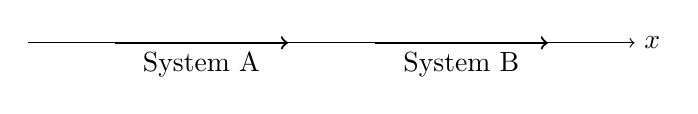
\begin{tikzpicture}[scale=1.1]
		
		% Achse
		\draw[->] (-0.5,0) -- (6.5,0) node[right] {$x$};
		
		% erstes System
		\draw[thick,->] (0.5,0) -- (2.5,0);
		\node[below] at (1.5,0) {System A};
		
		% zweites (verschobenes) System
		\draw[thick,->] (3.5,0) -- (5.5,0);
		\node[below] at (4.5,0) {System B};
		
	\end{tikzpicture}
\end{center}
Dieses Beispiel zeigt den Kern der Symmetrieidee: Ein Naturgesetz ist genau dann fundamental, wenn es unabhängig von willkürlichen Festlegungen wie Ort, Zeit oder Orientierung gilt. Symmetrien sind daher keine Zusatzannahmen, sondern ein Prüfstein für die Allgemeingültigkeit physikalischer Gesetze.





\subsection{Mathematik als universelles Strukturprinzip}

Die bisherigen Abschnitte haben gezeigt, dass Mathematik\index{Mathematik} nicht durch anschauliche Objekte, sondern durch abstrakte Strukturen\index{Struktur} arbeitet. Vektoren\index{Vektor} erhalten ihre Bedeutung durch den Raum\index{Raum}, in dem sie liegen, und Symmetrien\index{Symmetrie} offenbaren sich durch das, was unter Veränderungen\index{Veränderung} invariant\index{Invarianz} bleibt. Damit stellt sich eine weiterreichende Frage: Warum tauchen dieselben mathematischen Strukturen in so unterschiedlichen Bereichen der Natur\index{Natur} immer wieder auf?

Die Antwort liegt nicht in den einzelnen Phänomenen, sondern in ihrer gemeinsamen Struktur. Mathematik beschreibt nicht die stoffliche Beschaffenheit von Systemen, sondern die Beziehungen\index{Relation}, die zwischen ihren Elementen bestehen. Wenn unterschiedliche physikalische Prozesse denselben Beziehungsmustern folgen, erscheinen sie zwangsläufig in derselben mathematischen Form.

So begegnen identische Strukturen in der Mechanik\index{Mechanik}, der Elektrodynamik\index{Elektrodynamik} und der Quantenphysik\index{Quantenphysik}, obwohl die beschriebenen Objekte kaum unterschiedlicher sein könnten. Teilchenbahnen\index{Teilchenbahn}, Felder\index{Feld} oder Zustandsfunktionen\index{Zustandsfunktion} unterscheiden sich in ihrer Interpretation, nicht jedoch in der mathematischen Organisation. Die Universalität\index{Universalität} der Mathematik ist daher keine Überraschung, sondern eine Konsequenz ihrer strukturellen Arbeitsweise.

Diese Sichtweise kehrt eine verbreitete Intuition um. Mathematik ist nicht deshalb universell, weil sie besonders abstrakt oder formal ist. Sie ist universell, weil sie genau das beschreibt, was verschiedenen Systemen gemeinsam ist. Abstraktion\index{Abstraktion} entfernt nicht die Wirklichkeit\index{Wirklichkeit}, sondern isoliert ihre invarianten Eigenschaften.

\begin{DidacticBox}[Warum Mathematik universell ist]
	Mathematik beschreibt keine Dinge, sondern Strukturen.  
	Was dieselbe Struktur besitzt, folgt denselben mathematischen Gesetzen\index{Naturgesetz}.
	
	Unterschiedlich sind die Bedeutungen,  
	nicht die Form.
\end{DidacticBox}

Gerade in der modernen Physik\index{Moderne Physik} wird dieser Zusammenhang deutlich. Je weiter sich die Theorien von anschaulichen Bildern entfernen, desto stärker treten gemeinsame mathematische Muster hervor. Differentialgleichungen\index{Differentialgleichung}, Symmetrien und Erhaltungsprinzipien\index{Erhaltungsprinzip} verbinden scheinbar disparate Phänomene zu einem einheitlichen formalen Rahmen.

Diese Universalität ist nicht beliebig. Sie wirkt als strenges Auswahlkriterium für physikalische Theorien\index{Theorie}. Ein Gesetz, das von willkürlichen Koordinaten\index{Koordinate}, speziellen Orten\index{Ort} oder besonderen Beobachtern\index{Beobachter} abhängt, kann keinen fundamentalen Anspruch erheben. Erst wenn eine Beschreibung unabhängig von solchen Festlegungen ist, erfüllt sie das Kriterium struktureller Allgemeingültigkeit.

Damit erhält Mathematik eine neue Rolle. Sie ist nicht nur ein Werkzeug zur Beschreibung bereits bekannter Phänomene, sondern ein Leitfaden für mögliche Theorien. Was mathematisch inkonsistent\index{Konsistenz} oder strukturell instabil\index{Stabilität} ist, kann keine tragfähige Beschreibung der Natur liefern. Die Mathematik begrenzt damit nicht nur unser Wissen, sondern auch das, was überhaupt als physikalisch sinnvoll in Frage kommt.

In dieser Perspektive erscheint Mathematik als universelles Strukturprinzip. Sie ordnet nicht die Vielfalt der Erscheinungen, sondern legt den Rahmen fest, innerhalb dessen Erscheinungen überhaupt miteinander vergleichbar werden. Ihre Universalität beruht nicht auf inhaltlicher Allwissenheit, sondern auf struktureller Strenge.

Damit schließt sich der Gedankengang dieses Kapitels. Abstraktion und Struktur sind keine Hilfskonzepte, sondern die Grundlage dafür, dass Mathematik in so unterschiedlichen Bereichen der Natur dieselbe Sprache sprechen kann.

\subsection{Abstraktion als Weg zur Wirklichkeit}

Abstraktion\index{Abstraktion} gilt im alltäglichen Sprachgebrauch oft als Gegensatz zur Wirklichkeit\index{Wirklichkeit}. Was abstrakt ist, erscheint fern, theoretisch oder künstlich. In der Mathematik\index{Mathematik} und Physik\index{Physik} bedeutet Abstraktion jedoch etwas grundlegend anderes. Sie ist kein Entfernen von Realität, sondern ein gezieltes Herausfiltern dessen, was für das Verständnis wesentlich ist.

Bereits einfache physikalische Modelle\index{Modell} arbeiten abstrakt. Ein Körper wird als Punkt\index{Punkt} betrachtet, Reibung\index{Reibung} wird vernachlässigt, ideale Bedingungen\index{Idealisierung} werden angenommen. Diese Vereinfachungen sind keine Täuschungen, sondern bewusste Entscheidungen. Sie ermöglichen es, Strukturen\index{Struktur} sichtbar zu machen, die in der Komplexität realer Situationen verborgen bleiben würden.

Abstraktion wirkt dabei wie ein Vergrößerungsglas. Indem Nebeneffekte ausgeblendet werden, treten die grundlegenden Beziehungen\index{Relation} deutlicher hervor. Ein Modell ist nicht deshalb nützlich, weil es alles enthält, sondern weil es genau das Richtige weglässt. Die Wirklichkeit wird nicht kopiert, sondern strukturiert.

\begin{DidacticBox}[Abstraktion und Realität]
	Abstraktion bedeutet nicht Realitätsverlust.  
	Sie bedeutet Fokussierung.
	
	Was weggelassen wird, sind kontextabhängige Eigenschaften.  
	Was erhalten bleibt, ist die zugrunde liegende Struktur.
\end{DidacticBox}

Gerade die moderne Physik\index{Moderne Physik} zeigt die Notwendigkeit dieses Vorgehens. Quantenmechanik\index{Quantenmechanik}, Relativitätstheorie\index{Relativitätstheorie} und Feldtheorien\index{Feldtheorie} operieren mit Begriffen, die sich jeder unmittelbaren Anschauung entziehen. Dennoch liefern sie die präzisesten Vorhersagen\index{Vorhersage}, die die Physik kennt. Ihre Nähe zur Wirklichkeit zeigt sich nicht in Bildern, sondern in der Genauigkeit ihrer Aussagen.

Diese Entwicklung ist kein Zufall. Je tiefer man in die Struktur der Natur\index{Natur} eindringt, desto weniger tragen anschauliche Vorstellungen. Abstrakte Begriffe ersetzen konkrete Bilder, weil sie invariant\index{Invarianz} unter verschiedenen Darstellungen bleiben. Die Mathematik liefert genau diese invarianten Strukturen und macht sie unabhängig von subjektiver Wahrnehmung\index{Wahrnehmung}.

Abstraktion ist damit kein Umweg, sondern der direkte Weg zur Wirklichkeit. Sie ermöglicht es, allgemeine Gesetzmäßigkeiten\index{Naturgesetz} zu erkennen, die über einzelne Beobachtungen hinausgehen. Was zunächst fern erscheint, erweist sich bei genauer Betrachtung als das Verlässlichste, was wir über die Natur aussagen können.

In diesem Sinne bildet Abstraktion den Abschluss und zugleich den Übergang dieses Kapitels. Sie verbindet die mathematische Sprache der Natur mit ihrer strukturellen Ordnung und bereitet den Blick auf jene Bereiche vor, in denen Zufall\index{Zufall}, Wahrscheinlichkeit\index{Wahrscheinlichkeit} und Unsicherheit\index{Unsicherheit} eine zentrale Rolle spielen. Auch dort bleibt Mathematik kein Gegenpol zur Wirklichkeit, sondern ihr präzisestes Ausdrucksmittel.
